\documentclass[11pt]{article}

\usepackage[letterpaper,margin=0.75in]{geometry}
\usepackage{booktabs}
\usepackage{graphicx}
\usepackage{listings}
\usepackage{hyperref}

\setlength{\parindent}{1.4em}

\begin{document}

\lstset{
  language=Python,
  basicstyle=\small,          % print whole listing small
  keywordstyle=\bfseries,
  identifierstyle=,           % nothing happens
  commentstyle=,              % white comments
  stringstyle=\ttfamily,      % typewriter type for strings
  showstringspaces=false,     % no special string spaces
  numbers=left,
  numberstyle=\tiny,
  numbersep=5pt,
  frame=tb,
}

\newenvironment{absolutelynopagebreak}
  {\par\nobreak\vfil\penalty0\vfilneg
   \vtop\bgroup}
  {\par\xdef\tpd{\the\prevdepth}\egroup
   \prevdepth=\tpd}

\title{Network Simulation}

\author{Cody Heffner}

\date{22 Jan. 2015}

\maketitle

\section{Preface}

This report details the experiment I ran and the results obtained as specified by the Network Simulation Lab in the BYU CS 460 class taught by Dr. Zappala. The project specifications can be found \href{http://cs460.byu.edu/winter-2015/labs/network-simulation}{here}.

The experiment requires heavy use of a network simulator to test different network scenarios. The network simulator I used is Dr. Zappala's \href{https://github.com/zappala/bene}{Bene}, written in Python. All my simulation examples shown will be tailored towards use for that simulator.

\section{Summary}

The goal of the experiment was to test various network scenarios by sending packets across networks of diverse bandwidth and distances, then observing the delays incurred by the transmission, propogation, and queueing of those packets in the network. The next section describes an experiment in which a simple two-node network and one bi-directional link was set to various bandwidths and lengths. The following section reports a similar experiment with a three-node network and two bi-directional links. The section after that describes the portion of the experiment that was used to validate queueing theory with regards to an M/D/1 queue on a network. The final section summarizes the experiment as a whole and discusses a problem encountered during the experiment that gave me deeper insight into how the internet works.

\section{Two Nodes}

The network I created for this part of the experiment was a simple network consisting of two nodes and one bi-directional link. The following scenarios were tested:

\begin{enumerate}

\item One packet of length 1000 bytes sent from node n1 to node n2 at time 0. The network's bandwidth was 1Mbps with a propagation delay of 1 second.

\item One packet of length 1000 bytes sent from node n1 to node n2 at time 0. The network's bandwidth was 100bps with a propagation delay of 10 ms.

\item Three packets of length 1000 bytes sent from node n1 to node n2 at time 0, then one more packet sent at time 2. The network's bandwidth was 1Mbps with a propagation delay of 10 ms.

\end{enumerate}

The following two code blocks show how I set up the first scenario with one packet sent on a 1Mbps link and a propagation delay of 1. (Network setup for the other two scenarios are nearly exactly identical so I have omitted the code from this report.) The first block of code is a Python snippet interacting with the Bene simulator. Line 3 builds a Network object as described in the file 2n1.txt, which is shown in the second code block below. Lines 6 and 7 of sim.py simply retrieve nodes for later use. Lines 8 and 9 add a forwarding entry in its forwarding tables for the other node. For example on line 8 the function \emph{add\textunderscore forwarding\textunderscore entry} takes the parameters \emph{address} and \emph{link}. \emph{Address} can be thought of as the receiving IP address n2 has designated to receive packets from n1; thus, the code needs to retrieve that address from n2's attributes. The parameter \emph{link} represents the physical line going out from n1 to n2. In this case it is the first and only link enumerated within n1's \emph{link} array. The forwarding entry is added to n1's forwarding tables.

\vspace{5mm}
\begin{absolutelynopagebreak}
\begin{lstlisting}
# sim.py
    # setup network
    net = Network('networks/2n1.txt')

    # setup routes
    n1 = net.get_node('n1')
    n2 = net.get_node('n2')
    n1.add_forwarding_entry(address=n2.get_address('n1'),link=n1.links[0])
    n2.add_forwarding_entry(address=n1.get_address('n2'),link=n2.links[0])

    # setup app
    d = DelayHandler()
    net.nodes['n2'].add_protocol(protocol="delay",handler=d)
\end{lstlisting}
\end{absolutelynopagebreak}
\vspace{5mm}

The file 2n1.txt is relatively self-explanatory, but I'll go over it quickly. The first three lines are ignored. Lines 4 and 5 establish nodes and links between nodes. The first word represents a node to be created, and all following words on that same line represent a connection between the first word and each following word. Lines 8 and 9 configure links. The first two words target the start and end node of a link, and the last two words set that link to have a 1Mbps bandwidth and 1000ms (1 second) propagation delay.

\vspace{5mm}
\begin{absolutelynopagebreak}
\begin{lstlisting}
# 2n1.txt
    # n1 -- n2
    #
    n1 n2
    n2 n1

    # link configuration
    n1 n2 1Mbps 1000ms
    n2 n1 1Mbps 1000ms
\end{lstlisting}
\end{absolutelynopagebreak}
\vspace{5mm}

The simulator simulates three types of delays that packets experience as they travel: transmission, propagation, and queueing. 

Transmission delay is calculated as the result of the size of the packet in bits divided by the bandwidth of the link it is being transmitted onto. In scenario 1, transmission delay is the result of (8,000 bits / 1,000,000 bps) = 0.008s.

Propagation delay is simply a factor of the distance and speed the packet has to travel, but in this experiment, the propagation delays are given. In scenario 1, propagation delay = 1s

Queueing delay is how long a packet has to wait after it is fully received by a node. The cause of queueing delay is solely a factor of how many packets are in line at a node when a packet needs to be sent. In scenario 1, only one packet ever exists, so there will be no queueing delay.

The total delay is the sum of all three of those delays.

The following table shows each simulation's output of each packet's identifier, the time it was created, and the time it was received.

\vspace{0.5cm}
\begin{absolutelynopagebreak}
\begin{tabular}{lccc}
  \toprule
  Scenario & Packet ID & Time Created & Time Receieved\\
  \midrule
  First & 1 & 0s & 1.008s \\
  Second & 1 & 0s & 80.01s \\
  Third & 1 & 0s & 0.018s \\
  Third & 2 & 0s & 0.026s \\
  Third & 3 & 0s & 0.034s \\
  Third & 4 & 2s & 2.018s \\
  \bottomrule
  Raw Data
\end{tabular}
\end{absolutelynopagebreak}
\vspace{0.5cm}

The simulator can be shown as being accurate by comparing theoretical results with simulator results. The following tables compare the delay the packets experience in each situation traveling from n1 to n2 as calculated by hand and the delay the simulator reported the packets experienced. In any scenarios with multiple packets, I will show the queueing delay as experienced by the packet with the largest queueing delay.

\vspace{0.5cm}
\begin{absolutelynopagebreak}
\begin{tabular}{lcc}
  \toprule
  Delay Type & Calculated & Simulated\\
  \midrule
  Transmission & 0.008s & 0.008s\\
  Propagation & 1s & 1s\\
  Queue & 0s & 0s\\
  Total & 1.008s & 1.008s\\
  \bottomrule
  Scenario 1
\end{tabular}
\end{absolutelynopagebreak}
\vspace{0.5cm}

\begin{absolutelynopagebreak}
\begin{tabular}{lcc}
  \toprule
  Delay Type & Calculated & Simulated\\
  \midrule
  Transmission & 80s & 80s\\
  Propagation & 0.01s & 0.01s\\
  Queue & 0s & 0s\\
  Total & 80.01s & 80.01s\\
  \bottomrule
  Scenario 2
\end{tabular}
\end{absolutelynopagebreak}
\vspace{0.5cm}

\begin{absolutelynopagebreak}
\begin{tabular}{lcc}
  \toprule
  Delay Type & Calculated & Simulated\\
  \midrule
  Transmission & 0.008s & 0.008s\\
  Propagation & 0.01s & 0.01s\\
  Queue & 0.016s & 0.016\\
  Total & 0.034s & 0.034s\\
  \bottomrule
  Scenario 3
\end{tabular}
\end{absolutelynopagebreak}
\vspace{0.5cm}

In scenario 3, node n1 sends three packets back to back. N1 needs to place the third packet in a queue behind the other two while it transmits the first two. Therefore, the largest queueing delay will be experienced by the third packet and will be equal to two times the transmission delay for any packet.

As the three tables above show, the simulator is precise and accurate, finding each of the simulated delay values are equal to the calculated delay values. 

\section{Three Nodes}

For the three-node portion of the experiment, I set up three separate networks. The following list enumerates the three scenarios for which I needed separate networks. 

\begin{enumerate}

\item Two Fast Links, Part A: In a network consisting of three nodes A, B, and C, perform the transfer of a 1 MB file divided into 1000 1 kB packets from node A to C. The links include a link from A to B with 100 ms propagation delay and 1 Mbps bandwidth, and a link from B to C otherwise identical to the first link.

\item Two Fast Links, Part B: In a network consisting of three nodes A, B, and C, perform the transfer of a 1 MB file divided into 1000 1 kB packets from node A to C. The links include a link from A to B with 100 ms propagation delay and 1 Gbps bandwidth, and a link from B to C otherwise identical to the first link.

\item One Fast Link and One Slow Link: In a network consisting of three nodes A, B, and C, perform the transfer of a 1 MB file divided into 1000 1 kB packets from node A to C. The links include a link from A to B with 100 ms propagation delay and 1 Mbps bandwidth, and a link from B to C with 100 ms propagation delay and 256 Kbps bandwidth.

\end{enumerate}

By inspection, all these scenarios are nearly identical. I will only show the raw code for the first network. The following two code blocks show the .txt file describing the network to Bene and the Python file that executes the experiment.

\vspace{5mm}
\begin{absolutelynopagebreak}
\begin{lstlisting}
# 3n1a.txt
    # n1 -- n2 -- n3
    #
    n1 n2
    n2 n1 n3
    n3 n2

    # link configuration
    n1 n2 1Mbps 100ms
    n2 n1 1Mbps 100ms
    n2 n3 1Mbps 100ms
    n3 n2 1Mbps 100ms
\end{lstlisting}
\end{absolutelynopagebreak}

\vspace{5mm}

\begin{absolutelynopagebreak}
\begin{lstlisting}
# sim.py
    # setup network
    net = Network('networks/3n1a.txt')

    # setup routes
    n1 = net.get_node('n1')
    n2 = net.get_node('n2')
    n3 = net.get_node('n3')
    n1.add_forwarding_entry(address=n2.get_address('n1'),link=n1.links[0])
    n1.add_forwarding_entry(address=n3.get_address('n2'),link=n1.links[0])
    n2.add_forwarding_entry(address=n1.get_address('n2'),link=n2.links[0])
    n2.add_forwarding_entry(address=n3.get_address('n2'),link=n2.links[1])
    n3.add_forwarding_entry(address=n2.get_address('n3'),link=n3.links[0])
    n3.add_forwarding_entry(address=n1.get_address('n2'),link=n3.links[0])

    # setup app
    d = DelayHandler()
    net.nodes['n1'].add_protocol(protocol="delay",handler=d)
    net.nodes['n2'].add_protocol(protocol="delay",handler=d)
    net.nodes['n3'].add_protocol(protocol="delay",handler=d)
\end{lstlisting}
\end{absolutelynopagebreak}
\vspace{5mm}

Upon close inspection of sim.py, the network needs to be set up in a slightly different way than the two-node network. This network needed six different forwarding table entries compared with two entries in the two-node network. This is because there needs to be a forwarding table entry from \emph{each} node to \emph{every other} node. As you can see from the code, a forwarding table entry is added from n1 to n2 and to n3, then from n2 to n1 and to n3, then finally from n3 to n2 and to n1. The most interesting cases are from n1 to n3 and back. N1 doesn't have a direct link to n3, so it must go through n2. Thus, the forwarding table entry from n1 to n3 needs to specify that it needs to go to the address n3 has dedicated to receive from n2, and it needs to run on the first (and only) link n1 has - the link to n2. Beyond that, it is up to the implementation of the node class to know how to differentiate packets that have arrived at their destination and need to be forwarded.

In the first scenario of transferring a 1 MB file across a pretty fast network, the simulation calculated that the file transfer was complete at time t=8.208s. For the second scenario of transferring a 1 MB file across a very fast network, the simulation calculated that the file transfer was complete at time t=0.208008s. The unbalanced network scenario, where one link was fast and one link was slow, resulted in a file transfer time of t=31.458s.

\vspace{0.5cm}
\begin{absolutelynopagebreak}
\begin{tabular}{lcc}
  \toprule
  Scenario & File Transfer Time\\
  \midrule
  1 & 8.208s \\
  2 & 0.208008s \\
  3 & 31.458s \\
  \bottomrule
\end{tabular}
\end{absolutelynopagebreak}
\vspace{0.5cm}

These values correlate exactly with the answers I calculated in the first homework assignment. The equation used to calculate the delay of the first scenario with a pretty fast network is:

\vspace{5mm}
\begin{absolutelynopagebreak}
\begin{lstlisting}
t = (2*transmission + 2*propagation) + 999 * transmission
  = (2*(8000 bits / 1000000 bps) + 0.200s) + 999 * (8000 bits / 1000000 bps))
  = (0.216s) + 999 * 0.008s
t = 8.208s
\end{lstlisting}
\end{absolutelynopagebreak}
\vspace{5mm}

In this scenario, the first bit of the first packet is set on the line from n1 to n2 at t=0s. It travels to n2 in one \emph{propagation} delay length of time, arriving at n1 at t=100ms. It sits and waits at n2 for the trailing bits to arrive, which takes one duration of the \emph{transmission} delay. When the whole packet has arrived at n2, the first bit is sent on the line to n3 immediately, because there is no other packet ahead of it. It arrives at n3 in one more \emph{propagation} length of time (accounting for \emph{2*propagation} in the formula above), then must wait one more \emph{transmission} length of time (accounting for \emph{2*transmission} in the formula above). When the first packet is at n3, all other packets will be streaming in back-to-back at n3. The file transfer will be complete when n3 has received 999 more packets, all taking a duration equal to the \emph{transmission} delay to arrive.

In the second scenario, the same formula may be used as long as corrections are made to the transmission delay. The transmission delay in this scenario is 1000 times smaller because the link is 1000 times faster while the packet size and number of packets are equivalent. The only delay that doesn't shrink is the propagation delay - this stays the same as the first scenario.

In the third scenario, a new variable is introduced: the queueing delay. Because the second link has lower bandwidth, n2 will not be able to transmit packets as fast as it receives them. N2 will need to store incoming packets in a queue so that it will not lose packets if it's still busy transmitting other packets to n3. I derived the formula to calculate the queueing delay in my homework and will not re-derive it here. The following block shows the basic formula representing this scenario as well as the calculated answer, which is equal to the value received by the simulator.

\vspace{5mm}
\begin{absolutelynopagebreak}
\begin{lstlisting}
queue(n) = L(K-1)(1/Rslow - 1/Rfast)
t = 1000 * transfast + prop + queue(1000) + 1000 * transslow + prop
  = 1000 * 0.008s + 0.1s + 23.226750s + 1000 * 0.03125s + 0.1s
t = 31.458s
\end{lstlisting}
\end{absolutelynopagebreak}
\vspace{5mm}

\section{Queueing Theory}

The final part of my experiment was to validate queueing theory for an M/D/1 queue. An M/D/1 queue is a single queue that receives packets as an exponential distribution and services those packets deterministically. The following enumeration describes my process for this part of the experiment. The corresponding code is shown below the enumeration. 

\begin{enumerate}

\item I modified some existing code in Bene's \emph{delay.py} script. The only modifications I made were to run the simulation for a longer duration and to allow me to vary the utilization of the server's queue directly from the command line. The goal of this code is to throw packets at the node at random times, rather than predetermined like in previous experiments.

\item Next, I created a parser to average the queue time of each packet from \emph{delay.py}'s output. 

\item I then created a shell script to run all the simulations at once. 

\item Finally, I created a Python script to graph my results compared with the theoretical expected behavior.

\end{enumerate}

\vspace{5mm}
\begin{absolutelynopagebreak}
\begin{lstlisting}
# delay.py
    #arguments
    parser = argparse.ArgumentParser(prog='Delayed Packets')
    parser.add_argument('-u', '--util', type=float, action='store', default='all')
    args = parser.parse_args()
    utilization = args.util

    # parameters
    Sim.scheduler.reset()

    # setup network
    net = Network('../networks/one-hop.txt')

    # setup routes
    n1 = net.get_node('n1')
    n2 = net.get_node('n2')
    n1.add_forwarding_entry(address=n2.get_address('n1'),link=n1.links[0])
    n2.add_forwarding_entry(address=n1.get_address('n2'),link=n2.links[0])

    # setup app
    d = DelayHandler()
    net.nodes['n2'].add_protocol(protocol="delay",handler=d)

    # setup packet generator
    destination = n2.get_address('n1')
    max_rate = 1000000/(1000*8)

    load = utilization*max_rate
    g = Generator(node=n1,destination=destination,load=load,duration=1000)
    Sim.scheduler.add(delay=0, event='generate', handler=g.handle)
    
    # run the simulation
    Sim.scheduler.run()
\end{lstlisting}
\end{absolutelynopagebreak}

\vspace{5mm}

\begin{absolutelynopagebreak}
\begin{lstlisting}
# delayparser.py
    class Delayparser(object):
        def __init__(self):
            pass

        def parse(self, filename):
            f = open(filename, "r")

            avg = 0.0
            count = 0.0
            # skip the first line
            for line in f.readlines():
                if (line[0] != 'R' and line[0] != '\n'):
                    avg += float(line.split(' ')[6].split('\n')[0])
                    count += 1
            return [count, avg / count]

    if __name__ == '__main__':
        d = Delayparser()

        util = [10, 20, 30, 40, 50, 60, 70, 80, 90, 95, 98]

        for u in util:
            f = "outputs/qt_" + str(u) + ".txt"
            ret = d.parse(f)
            print "{:.0f}% utilization: {:.0f} packets, {:.6f} average queue delay.".format(u, ret[0], ret[1])
\end{lstlisting}
\end{absolutelynopagebreak}

\vspace{5mm}

\begin{absolutelynopagebreak}
\begin{lstlisting}
# delay.sh
    python delay.py -u 0.1 >> outputs/qt_10.txt
    python delay.py -u 0.2 >> outputs/qt_20.txt
    python delay.py -u 0.3 >> outputs/qt_30.txt
    python delay.py -u 0.4 >> outputs/qt_40.txt
    python delay.py -u 0.5 >> outputs/qt_50.txt
    python delay.py -u 0.6 >> outputs/qt_60.txt
    python delay.py -u 0.7 >> outputs/qt_70.txt
    python delay.py -u 0.8 >> outputs/qt_80.txt
    python delay.py -u 0.9 >> outputs/qt_90.txt
    python delay.py -u 0.95 >> outputs/qt_95.txt
    python delay.py -u 0.98 >> outputs/qt_98.txt

    python delayparser.py > outputs/average_queueing_delay.txt
\end{lstlisting}
\end{absolutelynopagebreak}

\vspace{5mm}

\begin{absolutelynopagebreak}
\begin{lstlisting}
# plot.py
    # Class that parses a file and plots several graphs
    class Plotter:
        def __init__(self):
            self.x = [0.1, 0.2, 0.3, 0.4, 0.5, 0.6, 0.7, 0.8, 0.9, 0.95, 0.98]
            self.y = [0.000463, 0.001016, 0.001702, 0.002650, 0.003899, 0.006066, 0.009240, 0.016074, 0.032784, 0.081299, 0.205917]

        def combinedPlot(self):
            """ Create a graph that includes a line plot and a boxplot. """
            clf()
            ax = plt.figure().add_subplot(111)

            # plot the data
            plot(self.x, self.y, label='Theory')

            # plot the equation
            # u = 125                           # service rate = 1/transmission delay = R / L
            p = np.arange(0, 0.995, 0.001)      # utilization
            y = []
            for i in range(0, len(p)):
                y.append(1.0/(2.0*125.0) * (p[i])/(1.0-(p[i])))
            plot(p, y, label='Average')

            # set up the axis
            xlabel('Utilization')
            ax.set_xticks(np.arange(0,1.1,0.1))
            ylabel('Average Queue Duration')
            ax.set_yticks(np.arange(0,0.7,0.1))

            # create a legend
            legend = ax.legend(loc='upper left', shadow=True)

            #print it out
            savefig('outputs/lab1_final.png')

    if __name__ == '__main__':
        p = Plotter()
        p.combinedPlot()
\end{lstlisting}
\end{absolutelynopagebreak}
\vspace{5mm}

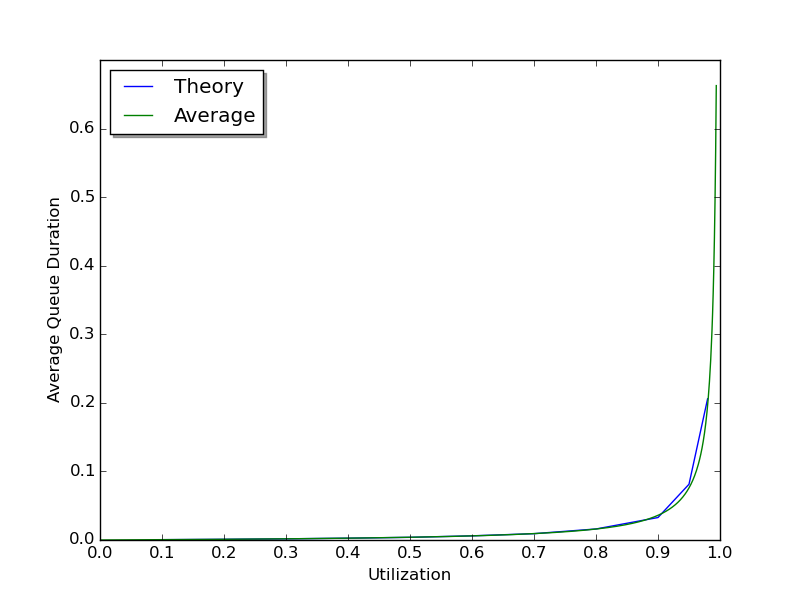
\includegraphics[width=17cm]{outputs/lab1_final.png}

The final result is a graph showing the relationship between the theoretical and actual queueing delay produced by the simulator. The correlation between theory and observed is extremely high. 

\section{Conclusion}

This experiment confirmed the behavior of the internet that we have learned about so far in CS 460 - that is, it confirmed how propagation, transmission, and queueing delays work, and that queueing theory is valid with an M/D/1 queue.

During the queueing theory portion of the experiment I ran into some trouble that gave me deeper insight on how the internet works. I left the duration to throw packets at the server at 10 seconds. This made my data vary \emph{greatly}, to the point where higher utilization levels weren't anywhere near the theoretical curve. I attempted to run this experiment multiple times to get more data points to average. This improved my data slightly but not to the point where I'd feel comfortable saying this experiment verified queueing theory. After looking through the code, I changed the duration from 10 to 100 seconds. This led to significant improvement. I increased it further to 1000 and got the results shown above. 

I pondered why running the experiment multiple times would not improve results but increasing the duration would. I came to the conclusion that by running multiple iterations, I was allowing the server's queue to clear. Just by periodically allowing the server's queue to clear every 10 seconds, the queue time at higher utilizations was reduced more than 50\%.

This could be an interesting area of research for another time: what is the relationship between periodic breaks and queue times at various utilizations? How high can utilization of servers be pushed if they are periodically allowed breaks? Would this be more efficient or effective than keeping utilizations low?

\end{document}
